\documentclass{article}
\usepackage{fullpage,amsmath,amssymb}
\usepackage{hyperref}
\usepackage{tikz}
\usetikzlibrary{arrows, automata,positioning}
\title{CSC236H, Fall 2017\\
Assignment 3\\
Due December 7th, 11:55 p.m.}
\renewcommand{\today}{~}
\hypersetup{pdfpagemode=Fullscreen,
  colorlinks=true,
  linkfileprefix={}}

\newcommand{\floor}[1]{\lfloor #1 \rfloor}

\begin{document}
\maketitle
\vspace{-1.5cm}
\begin{itemize}
  \item You may work in groups of no more than \textbf{three} students, and you should
  produce a single solution in a PDF file named \texttt{a3.pdf}, submitted to {MarkUs}.
    Submissions must be \textbf{typed}.
  \item Please refer to the course information sheet for the \textbf{late submission policy}.
\end{itemize}
\vspace{1\baselineskip}

\begin{enumerate}
  \item For each of the following languages give a regular expression that generates the language. You do not need to prove that your regular expression is correct.
       \begin{enumerate}
       \item $L = \{x \in \{0, 1\}^*: x$ starts with 0 and does not contain substring 101$\}$
       \\ solution: 00*1*(0* + 001*)*
       \item $L = \{x \in \{0, 1\}^*: x$ does not start with 00 and does not end with 11 $\}$
       \\solution: (11+10+01)(0+1)*(01+10)+($\epsilon$+ 0 + 1)+(01+10)+(101+100+110+010)
       \end{enumerate}
    \item Give an NFA for the following language
      $$L = \{w\in\{0,1\}^\ast : w \mbox{ is 0-alternating}\}$$
      A binary string $w$ is said to be 0-alternating iff either all the symbols in odd positions within $w$ are 0's,
      or all the symbols in even positions within $w$ are 0's, or both.\\
      For example, if $w$ = $b_1b_2b_3b_4b_5$, where each $b_i \in \{0, 1\}$,
      then $w$ is 0-alternating iff either $b_1 = b_3 = b_5 = 0$, or $b_2 = b_4 = 0$,
      or $b_1 = b_2 = b_3 = b_4 = b_5 = 0$.\\
      Note that any string of length less than 2 is 0-alternating. \\

      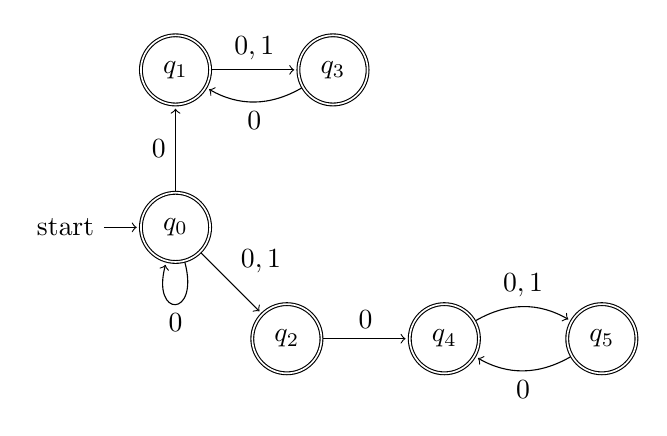
\begin{tikzpicture}[shorten >=1pt,node distance=2cm,on grid,auto]
        \node[state, initial, accepting] (q_0)   {$q_0$};
        \node[state, accepting] (q_1) [above=of q_0] {$q_1$};
        \node[state, accepting] (q_2) [below right=of q_0] {$q_2$};
        \node[state, accepting] (q_3) [right=of q_1] {$q_3$};
        \node[state, accepting] (q_4) [right=of q_2] {$q_4$};
        \node[state, accepting] (q_5) [right=of q_4] {$q_5$};
        \path[->] (q_0) edge [loop below] node {$0$} (q_0);
        \path[->] (q_0) edge  node  {$0$} (q_1);
        \path[->] (q_1) edge  node {$0, 1$} (q_3);
        \path[->] (q_2) edge  node {$0$} (q_4);
        \path[->] (q_0) edge node {$0, 1$} (q_2);
        \path[->] (q_3) edge [bend left] node {$0$} (q_1);
        \path[->] (q_4) edge [bend left] node {$0, 1$} (q_5);
        \path[->] (q_5) edge [bend left] node {$0$} (q_4);
      \end{tikzpicture}

  \item Construct the \textbf{smallest} DFA for each of the following languages.
    One mark will be deducted for each extra state that your DFA uses.\\
    Provide appropriate \textbf{state invariants} for each DFA.
    Do not use regular expressions in your state invariant.\\
     \begin{enumerate}
      \item $L = \{w \in \{0,1 \}^*:$ number of 0's in $w$ is divisible by 3 and $w$
      does not contain the substring 010 $\}$

      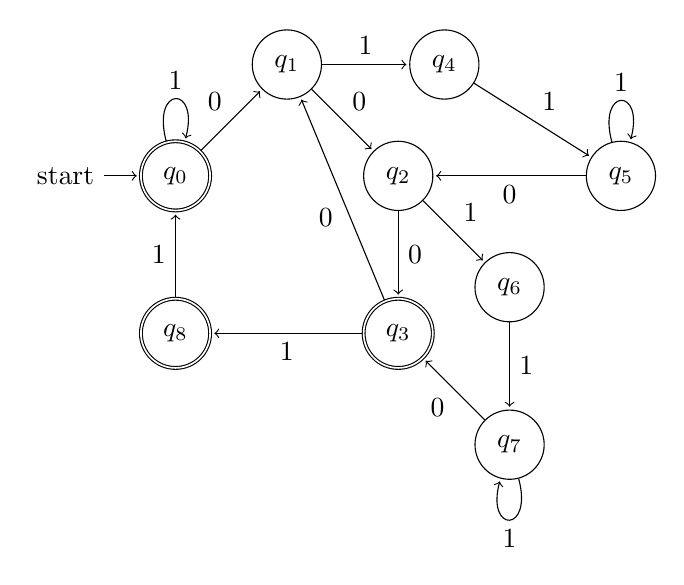
\begin{tikzpicture}[shorten >=1pt,node distance=2cm,on grid,auto]
        \node[state, initial, accepting] (q_0)   {$q_0$};
        \node[state] (q_1) [above right=of q_0] {$q_1$};
        \node[state] (q_2) [below right=of q_1] {$q_2$};
        \node[state, accepting] (q_3) [below=of q_2] {$q_3$};
        \node[state] (q_4) [right=of q_1] {$q_4$};
        \node[state] (q_6) [below right=of q_2] {$q_6$};
        \node[state] (q_5) [above right=of q_6] {$q_5$};
        \node[state] (q_7) [below=of q_6] {$q_7$};
        \node[state, accepting] (q_8) [below= of q_0] {$q_8$};
        \path[->] (q_0) edge  node {0} (q_1);
        \path[->] (q_0) edge  [loop above] node {1} ();
        \path[->] (q_1) edge  node {0} (q_2);
        \path[->] (q_1) edge  node {1} (q_4);
        \path[->] (q_2) edge  node {0} (q_3);
        \path[->] (q_2) edge  node {1} (q_6);
        \path[->] (q_3) edge  node {0} (q_1);
        \path[->] (q_3) edge  node {1} (q_8);
        \path[->] (q_4) edge  node {1} (q_5);
        \path[->] (q_5) edge  [loop above] node {1} ();
        \path[->] (q_5) edge  node {0} (q_2);
        \path[->] (q_6) edge  node {1} (q_7);
        \path[->] (q_7) edge  [loop below] node {1} ();
        \path[->] (q_7) edge  node {0} (q_3);
        \path[->] (q_8) edge  node {1} (q_0);
      \end{tikzpicture}

      $ \delta^\ast(q_0, w) = q_0 \mbox{ iff } $ \\
      i) (The number of 0s in w) mod 3 = 0 \\
      ii) (w ends in 11) or (w is 1) or (w is $\epsilon$) \\

      $ \delta^\ast(q_0, w) = q_1 \mbox{ iff } $ \\
      i) (The number of 0s in w) mod 3 = 1 \\
      ii) w ends in 0 \\

      $ \delta^\ast(q_0, w) = q_2 \mbox{ iff } $ \\
      i) (The number of 0s in w) mod 3 = 2 \\
      ii) w ends in 0 \\

      $ \delta^\ast(q_0, w) = q_3 \mbox{ iff } $ \\
      i) (The number of 0s in w) mod 3 = 0 \\
      ii) w ends in 0 \\

      $ \delta^\ast(q_0, w) = q_4 \mbox{ iff } $ \\
      i) (The number of 0s in w) mod 3 = 1 \\
      ii) w ends in 01 \\

      $ \delta^\ast(q_0, w) = q_5 \mbox{ iff } $ \\
      i) (The number of 0s in w) mod 3 = 1 \\
      ii) w ends in 11 \\

      $ \delta^\ast(q_0, w) = q_5 \mbox{ iff } $ \\
      i) (The number of 0s in w) mod 3 = 2 \\
      ii) w ends in 01 \\

      $ \delta^\ast(q_0, w) = q_5 \mbox{ iff } $ \\
      i) (The number of 0s in w) mod 3 = 2 \\
      ii) w ends in 11 \\

      $ \delta^\ast(q_0, w) = q_5 \mbox{ iff } $ \\
      i) (The number of 0s in w) mod 3 = 0 \\
      ii) w ends in 01 \\


      \item $L = \{x\in \{0,1\}^\ast : 00 \mbox{ is a substring of } x, \mbox{ but } 11 \mbox{ is not}\}$\\
      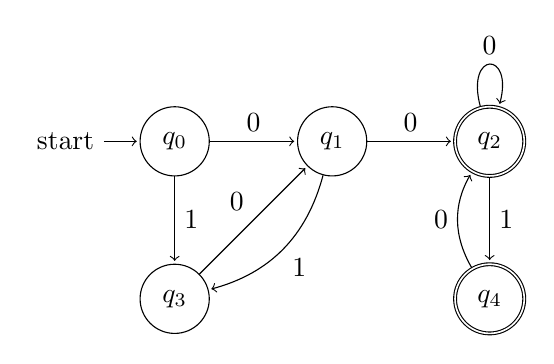
\begin{tikzpicture}[shorten >=1pt,node distance=2cm,on grid,auto]
        \node[state, initial] (q_0)   {$q_0$};
        \node[state] (q_1) [right=of q_0] {$q_1$};
        \node[state, accepting] (q_2) [right=of q_1] {$q_2$};
        \node[state] (q_3) [below=of q_0] {$q_3$};
        \node[state, accepting] (q_4) [below=of q_2] {$q_4$};
        \path[->] (q_0) edge  node {0} (q_1);
        \path[->] (q_0) edge  node {1} (q_3);
        \path[->] (q_1) edge  node {0} (q_2);
        \path[->] (q_1) edge  [bend left] node {1} (q_3);
        \path[->] (q_2) edge  [loop above] node {0} ();
        \path[->] (q_2) edge  node {1} (q_4);
        \path[->] (q_3) edge  node {0} (q_1);
        \path[->] (q_4) edge  [bend left] node {0} (q_2);
      \end{tikzpicture}

      \[\delta^\ast(q_0, w) =
      \begin{cases}
        q_1 & \mbox{ iff } w \ ends \ with \ 1 \ and \ 00 \ is \ not \ a \ substring \ of \ w \\
        q_2 & \mbox{ iff } w \ ends \ with \ 1 \ and \ 00 \ is \ a \ substring \ of \ w \\
        q_3 & \mbox{ iff } w \ ends \ with \ 0 \ and \ 00 \ is \ not \ a \ substring \ of \ w \\
        q_4 & \mbox{ iff } w \ ends \ with \ 0 \ and \ 00 \ is \ a \ substring \ of \ w \\
      \end{cases}
      \]
      The initial state is $q_0$. The only accepting states are $q_2$ and $q_4$.

     \end{enumerate}


    \newpage
    \item Let $\Sigma$ be an arbitrary alphabet. For every $w\in\Sigma^\ast$
    \[\rho(w) =
    \begin{cases}
      \epsilon  & \mbox{ if } w = \epsilon\\
        cx & \mbox{ if } w = xc \mbox{ for some }  x\in \Sigma^\ast \mbox{ and } c\in \Sigma\\
    \end{cases}
    \]

    Informally, for a nonempty string $w\in\Sigma^\ast$, $\rho(w)$ is the string obtained by
    moving the last symbol in $w$ to the first position.\\

    For every language $L\subseteq\Sigma^\ast$, we define
    $$Rotate(L) = \{x\in \Sigma^\ast: x =\rho(y) \mbox{ for some } y\in L\}.$$
    Prove that if $L$ is a regular language, then so is $Rotate(L)$.\\
    More specifically, you must show the \textbf{construction of a DFA} for $Rotate(L)$, and prove the
    correctness of the DFA.\\

    For this question, you may use the following fact about $\delta^\ast$ without proof:
    \begin{itemize}
  \item If $w=ax$, for some $x\in \Sigma^\ast$ and $a\in\Sigma$, then
  \[\delta^\ast(q, w) = \delta^\ast(\delta(q, a), x).\]
    \\
    \end{itemize}
    Assume $L$ is a regular language. Then exist a DFA  $\zeta_1$ that only accepts $L$\\
    Let $\zeta_1 = \left< Q_1,\Sigma_1,\delta_1,s_1,F_1 \right>$\\
    Let's define another DFA $\zeta_2 = \left< Q_2,\Sigma_2,\delta_2,s_2,F_2 \right>$ in the following way:\\
    $Q_2 = Q_1 \cup \{s_2\}$\\
    $\Sigma_2 = \Sigma_1$\\
    For $\forall q \in Q_2$ and $\forall w \in \Sigma_2$ or $w = \epsilon$
     $$\delta_2(q, w) =
        \begin{cases}
        s_2, $  if $ q = s_2 $ and $ w =\epsilon\\
        s_1, $  if $ q = s_2 \\
        \delta_1(q, w), $  else $\\
        \end{cases}$$
    Define $F_2$ in the following way:\\
    For $\forall q \in Q_2$, $q \in F_2$ iff $\exists x\in \Sigma_2^\ast$, $\exists y\in \Sigma_2$ such that $\delta_1^\ast(s_1, x) = q$ and $\delta_1(q, y) \in F_1$ or $\delta_1^\ast(s_1, \epsilon) \in F_1$ and $\delta_2^\ast(s_2, \epsilon) = q$ \\\\
    Claim: $\forall w \in \Sigma_2^\ast$, $P(w): \delta_2^\ast(s_1, w) = \delta_1^\ast(s_1, w) $\\
    \textbf{Base Case:} Let $w = \epsilon$\\
    Then $\delta_2^\ast(s_1, w) =s_1$ and $\delta_1^\ast(s_1, w) = s_1$\\
    Then $P(w)$ holds.\\
    \textbf{Induction step:} Let $w = xa$ for $x \in \Sigma_2^\ast$ and $a \in \Sigma_2$. Assume that $P(x)$ holds.[\textbf{IH}]\\
    Then $\delta_2^\ast(s_1, w) = \delta_2^\ast(s_1, xa) = \delta_2(\delta_2^\ast(s_1, x), a) $\\
    Then $\delta_2^\ast(s_1, w) = \delta_2(\delta_1^\ast(s_1, x), a)$ [\textbf{IH}]\\
    Then $\delta_2^\ast(s_1, w) = \delta_1(\delta_1^\ast(s_1, x), a)=\delta_1^\ast(s_1, w)$\\
    Thus $P(w)$ holds.\\\\
    Claim: For $\forall w \in \Sigma_2^\ast$ ,  $w \in Rotate(L)$  iff  $\delta_2^\ast(s_2, w) \in F_2$\\
    Let $w \in \Sigma_2^\ast$ \\
    Then  $w \in Rotate(L)$ iff $w = \rho(y)$ for some $y \in L$\\
    Then  $w \in Rotate(L)$ iff $\delta_1^\ast(s_1, y) \in F_1$\\
    We have two cases:\\
    \textbf{Case 1}:Let $y = xa$ for $x \in \Sigma_2^\ast$ and $a \in \Sigma_2$\\
    Then $w \in Rotate(L)$ iff $\delta_1^\ast(s_1, xa) \in F_1$\\
    Then $w \in Rotate(L)$ iff $\delta_1(\delta_1^\ast(s_1, x), a) \in F_1$\\
    Then $w \in Rotate(L)$ iff $\delta_1^\ast(s_1, x) \in F_2$\\
    Then $w \in Rotate(L)$ iff $\delta_2^\ast(s_1, x) \in F_2$\\
    Then $w \in Rotate(L)$ iff $\delta_2^\ast(\delta_2(s_2,a), x) \in F_2$\\
    Then $w \in Rotate(L)$ iff $\delta_2^\ast(ax) \in F_2$\\
    Then $w \in Rotate(L)$ iff $\delta_2^\ast(\rho(y)) \in F_2$\\
    Then $w \in Rotate(L)$ iff $\delta_2^\ast(w) \in F_2$\\
    \textbf{Case 2}: Let $y = \epsilon$\\
    Then $w \in Rotate(L)$ iff $\delta_1^\ast(s_1, \epsilon) \in F_1$\\
    Then $w \in Rotate(L)$ iff $\delta_2^\ast(s_2, \epsilon) \in F_2$\\
    Then $w \in Rotate(L)$ iff $\delta_2^\ast(s_2, \rho(y)) \in F_2$\\
    Therefore $\forall w \in \Sigma_2^\ast$ ,  $w \in Rotate(L)$  iff  $\delta_2^\ast(s_2, w) \in F_2$\\
    Thus $\zeta_2$ only accepts $Rotate(L)$\\
    Thus $Rotate(L)$ is a regular language.


    \item Let $L_1, L_2\subseteq \{b,c,0\}^\ast$ and
    \[L_1=\{w_10w_2: w_1,w_2\in\{b,c\}^\ast \mbox{ and } w_1=w_2\}\]
    Suppose we know that $L_1$ is not regular. \\
    Use \textbf{closure properties} of regular languages to prove that the language
    \[L_2=\{w_10w_2: w_1,w_2\in\{b,c\}^\ast \mbox{ and } w_1\neq w_2\}\]
    is not regular.\\\\
    Assume that $L_2$ is regular.\\
    Consider $L_1\cup L_2 = \{w_10w_2: w_1,w_2\in\{b,c\}^\ast\}$\\
    Claim: $L_1\cup L_2$ is a regular language.\\
    If there exist a DFA that accepts $L_1\cup L_2$ then $L_1\cup L_2$ is a regular language.\\\\
    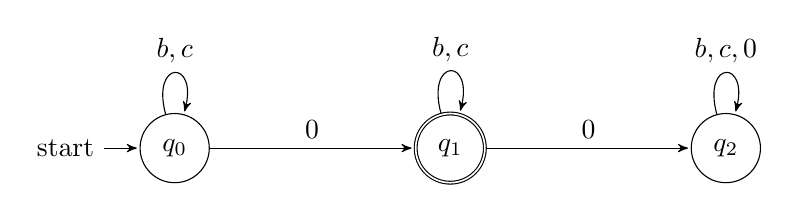
\begin{tikzpicture}[->,>=stealth',shorten >=1pt,auto,node distance=3.5cm,
        scale = 1,transform shape]

    \node[state,initial] (0) {$q_0$};
    \node[state,accepting] (1) [right of=0] {$q_1$};
    \node[state] (2) [right of=1] {$q_2$};

    \path (0) edge              node {$0$} (1)
        (0) edge    [loop above]          node {$b,c$} (0)
        (1) edge     [loop above]         node {$b,c$} (1)
        (1) edge            node{$0$}(2)
        (2) edge [loop above] node{$b,c,0$} (2);


    \end{tikzpicture}\\
    Let DFA $\zeta = \left< Q,\Sigma,\delta,q_0,F \right> $\\ where:\\
    $Q = \{q_0, q_1\}$ , $F = \{q_1\}$ , $\Sigma = \{b,c, 0\}$\\
    $\delta(q_0, b) = q_0, \quad \delta(q_0, c) = q_0, \quad \delta(q_0, 0) = q_1$\\
    $\delta(q_1, c) = q_1, \quad \delta(q_1, b) = q_1, \quad\delta(q_1, 0) = q_2$\\
    $\delta(q_2, b) = q_2, \quad \delta(q_2, c) = q_2, \quad \delta(q_2, 0) = q_2$\\
    Claim: $w \in L_1\cup L_2$ iff $\delta^\ast(q_0, w) \in F$\\
    Let $P(w)$ denote the assertion that
    $$\delta^\ast(q_0, w) =
        \begin{cases}
        q_0, $ if $ w $ does not have 0$\\
        q_1, $ if $ w $ has only one 0$\\
        q_2, $ if $ w $ two or more 0$
        \end{cases}$$

    \textbf{Base Case}: Let $w=\epsilon$\\
    Then $w$ has no 0\\
    Also $\delta^\ast(q_0, w) = q_0$, by the base rule definition of $\delta^\ast$\\
    $P(w)$ holds.\\
    \textbf{IS}: Suppose $w=xa$ for some $x \in \{b,c,0\}^\ast\ $ and $a \in \{b,c,0\}$. Assume $P(x)$ holds. [\textbf{IH}]\\
    \textbf{Case 1:} Assume $a \in \{b,c\}$\\
    \textbf{Case 1.1:} Assume $x$ has no 0.\\
    Then, $w$ has no 0.\\
    $\delta^\ast(q_0, w) = \delta(\delta^\ast(q_0, x), a)$ by definition of $\delta^\ast$\\
    $\delta^\ast(q_0, w) = \delta(q_0, a)$ by [IH]\\
    $\delta^\ast(q_0, w) = q_0$ by definition of $\delta$\\
    $P(w)$ holds.\\
    \textbf{Case 1.2:} Assume $x$ has one 0.\\
    Then, $w$ still has one 0.\\
    $\delta^\ast(q_0, w) = \delta(\delta^\ast(q_0, x), a)$ by definition of $\delta^\ast$\\
    $\delta^\ast(q_0, w) = \delta(q_1, a)$ by [IH]\\
    $\delta^\ast(q_0, w) = q_1$ by definition of $\delta$\\
    $P(w)$ holds.\\
    \textbf{Case 1.3:} Assume $x$ has two or more 0.\\
    Then, $w$ still has two or more 0.\\
    $\delta^\ast(q_0, w) = \delta(\delta^\ast(q_0, x), a)$ by definition of $\delta^\ast$\\
    $\delta^\ast(q_0, w) = \delta(q_2, a)$ by [IH]\\
    $\delta^\ast(q_0, w) = q_2$ by definition of $\delta$\\
    $P(w)$ holds.\\
    \textbf{Case 2:} Assume $a = 0 $\\
    \textbf{Case 2.1:}Assume $x$ has no 0.\\
    Then , $w$ has one 0.\\
    $\delta^\ast(q_0, w) = \delta(\delta^\ast(q_0, x), a)$ by definition of $\delta^\ast$\\
    $\delta^\ast(q_0, w) = \delta(q_0, a)$ by [IH]\\
     $\delta^\ast(q_0, w) = q_1$ by definition of $\delta$\\
    $P(w)$ holds.\\
    \textbf{Case 2.2:}Assume $x$ has one 0.\\
    Then , $w$ has two or more 0.\\
    $\delta^\ast(q_0, w) = \delta(\delta^\ast(q_0, x), a)$ by definition of $\delta^\ast$\\
    $\delta^\ast(q_0, w) = \delta(q_2, a)$ by [IH]\\
    $\delta^\ast(q_0, w) = q_2$ by definition of $\delta$\\
    $P(w)$ holds.\\
    \textbf{Case 2.3:}Assume $x$ has two or more 0.\\
    Then , $w$ has two or more 0.\\
    $\delta^\ast(q_0, w) = \delta(\delta^\ast(q_0, x), a)$ by definition of $\delta^\ast$\\
    $\delta^\ast(q_0, w) = \delta(q_2, a)$ by [IH]\\
    $\delta^\ast(q_0, w) = q_2$ by definition of $\delta$\\
    $P(w)$ holds.\\\\
    Thus $P(w)$ holds for $\forall w \in \{b,c,0\}^\ast$ \\\\
    Assume $w \in L_1\cup L_2$. Then $w$ has one 0.\\
    Since $P(w)$ holds, $\delta^\ast(q_0, w) = q_1$\\
    Since $q_1 \in F$, $\delta^\ast(q_0, w) \in F$\\\\
    Conversely, assume $\delta^\ast(q_0, w) \in F$\\
    Since $q_1$ is the only accepting state of $\zeta$, $\delta^\ast(q_0, w) = q_1$\\
    Assume for contradiction that $w \notin L_1\cup L_2$\\
    Then $w$ has no 0 or two or more 0.\\
    If $w$ has no 0, $\delta^\ast(q_0, w) = q_0$ by $P(w)$\\
    If $w$ has two or more 0, $\delta^\ast(q_0, w) = q_2$ by $P(w)$.\\
    In either case, $\delta^\ast(q_0, w) \neq q_1$, which leads to contradiction.\\
    Then $w \in L_1\cup L_2$\\
    Thus $L_1\cup L_2$ is a regular language.\\
    Then $\overline{(L_1\cup L_2)}$ is a regular language.\\
    Then $\overline{(L_1\cup L_2)} \cup L_2$ is a regular language since $L_2$ is a regular language\\
    Then $\overline{\overline{(L_1\cup L_2)} \cup L_2} = (L_1 \cup L_2) \cap \overline{L_2}$ is regular language.\\
    Then $(L_1 \cup L_2) \cap \overline{L_2}= (\overline{L_2} \cap L_2) \cup (\overline{L_2} \cap L_1) = (\overline{L_2} \cap L_1) $ is a regular language.\\\\
    Claim: $L_1 \subseteq \overline{L_2}$\\
    Let $w \in L_1$, then $w \notin L_2$\\
    Then $w \in \overline{L_2}$\\
    Therefore $L_1 \subseteq \overline{L_2}$
    Then $(\overline{L_2} \cap L_1) = L_1$ is a regular language.\\
    This leads to contradiction.
    Thus $L_2$ is not a regular language.





\end{enumerate}

\end{document}
